\documentclass[a4paper,12pt]{article}

\usepackage{titlesec}
\usepackage{enumitem}
\usepackage{geometry}
\usepackage{graphicx}

\geometry{a4paper, margin=1in}

\title{Space Pizza: Galactic Grooves}
\author{Eduard Pokhylko & Co.}
\date{\today}

\begin{document}
\section{Introduction}
This document outlines the project proposal for "Space Pizza Delivery," a computer graphics endeavor inspired by the aesthetics of 2000s games, particularly Jet Set Radio. The game involves a spacecraft on a mission to deliver pizzas to cartoonish planets within a stylized, simplified cosmic environment.

\section{Overview}
\subsection{Objective}
The primary goal of the game is to efficiently transport pizzas from a space pizza cafes to various planets  across the solar system. Players will accumulate points based on successful and timely deliveries.

\subsection{Visual Style}
Taking cues from the graphical style of Jet Set Radio, the game features a cartoonish and simplified aesthetic. However, it is important to us to fully implement all of the useful visual features of advanced OpenGL. Expect vivid colors, stylized environments, and an overall 2000's ambiance.

\subsection{Game World}
The game is set in a vast, whimsical solar system where individual cosmic objects serve as unique delivery destinations. The planetary scale is exaggerated to enhance the fantastical and playful atmosphere.

\subsection{Music}
An important part of the experience is the presence of a hip soundtrack that complements the funny adventure. The music reflects the overall style of the game, contributing to an engaging gaming experience.

\subsection{Mission Structure}
While the final mission remains undisclosed, players will engage in a series of progressively challenging pizza deliveries. Successful completion of each delivery brings them closer to uncovering the overarching narrative, adding an element of suspense and progression.

\pagebreak

\section{Graphics Techniques}
First and foremost, the implementation of CelShading, to define visual style.
Sprite rendering to support an informative GUI.
\begin{itemize}
    \item \textbf{Cel-shading:} Utilizing cel-shading technique to define a distinct rendering style. This involves outlining objects with bold, stylized lines to emulate a hand-drawn appearance.
  
    \item \textbf{Sprite Rendering:} Implementing sprite rendering for an informative GUI. This technique enables efficient rendering of textured 2D images in a 3D environment, contributing to the game's overall visual charm.
    
    \item \textbf{Physically Based Rendering (PBR):} Implementing PBR to achieve more realistic lighting and material properties. PBR simulates the interaction of light with surfaces based on their physical properties, enhancing the visual fidelity of materials.

    \item \textbf{Bloom:} Applying a bloom effect to enhance the visual appeal!
  
    \item \textbf{Normal Mapping:} Utilizing normal mapping to enhance surface details by simulating finer geometry without the need for additional polygons.

    \item \textbf{Parallel transport frames:} WIP.

\end{itemize}

\section{Chosen CG Method}
\subsection*{Volumetric Light Scattering}
Exploring the option of volumetric light scattering to simulate lighting effects through atmospheric elements. In other words, an effect present after consuming pizza (green fog around the planet)

\section*{Visual Appeal}
WIP.

\section*{Interactivity}
WIP.

\section*{Timeline}
For now, the project is in the stage of conception. We are working on creating a theme and general idea.

\section*{Conclusion}
TO BE DONE IN FUTURE TIME.

\subsection*{Style references:}
\begin{table}[h]
    \centering
    \begin{tabular}{|c|c|}
      \hline
      \textbf{Reference Image} & \textbf{Description} \\
      \hline
      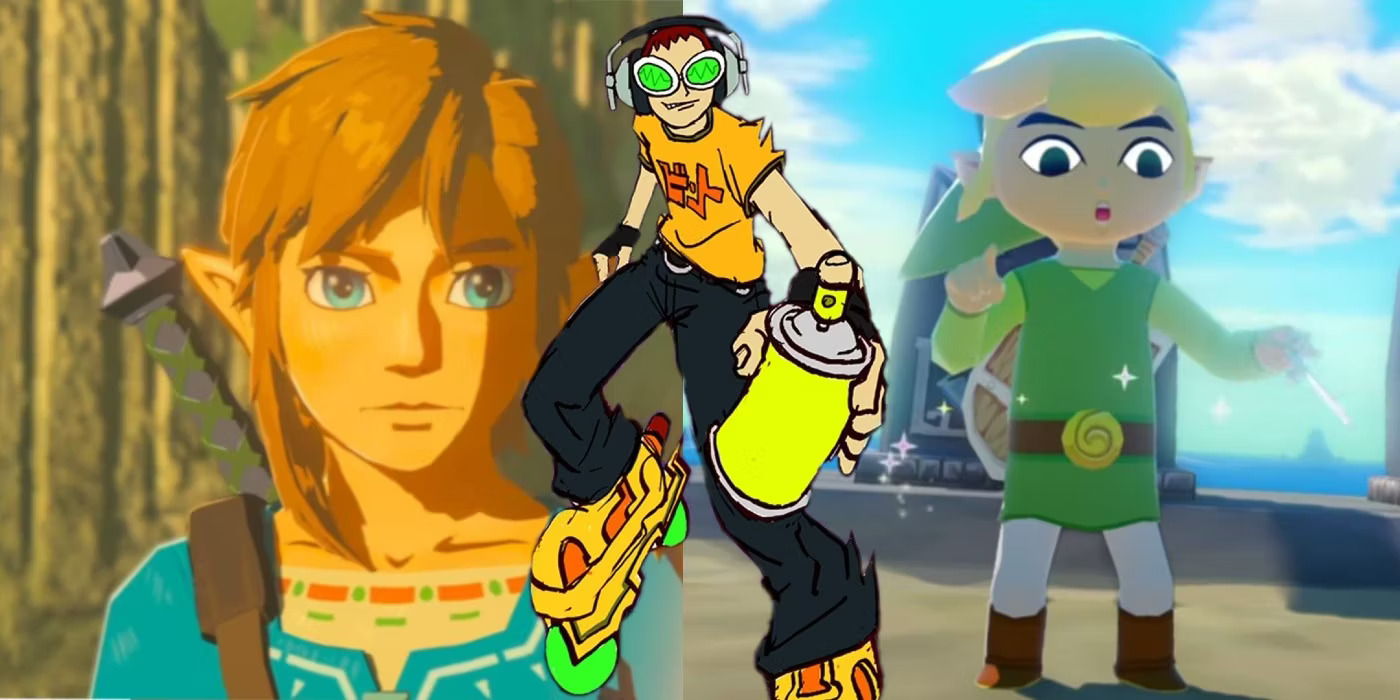
\includegraphics[width=0.4\linewidth]{image1.jpg} & Simplify the computation \\
      \hline
      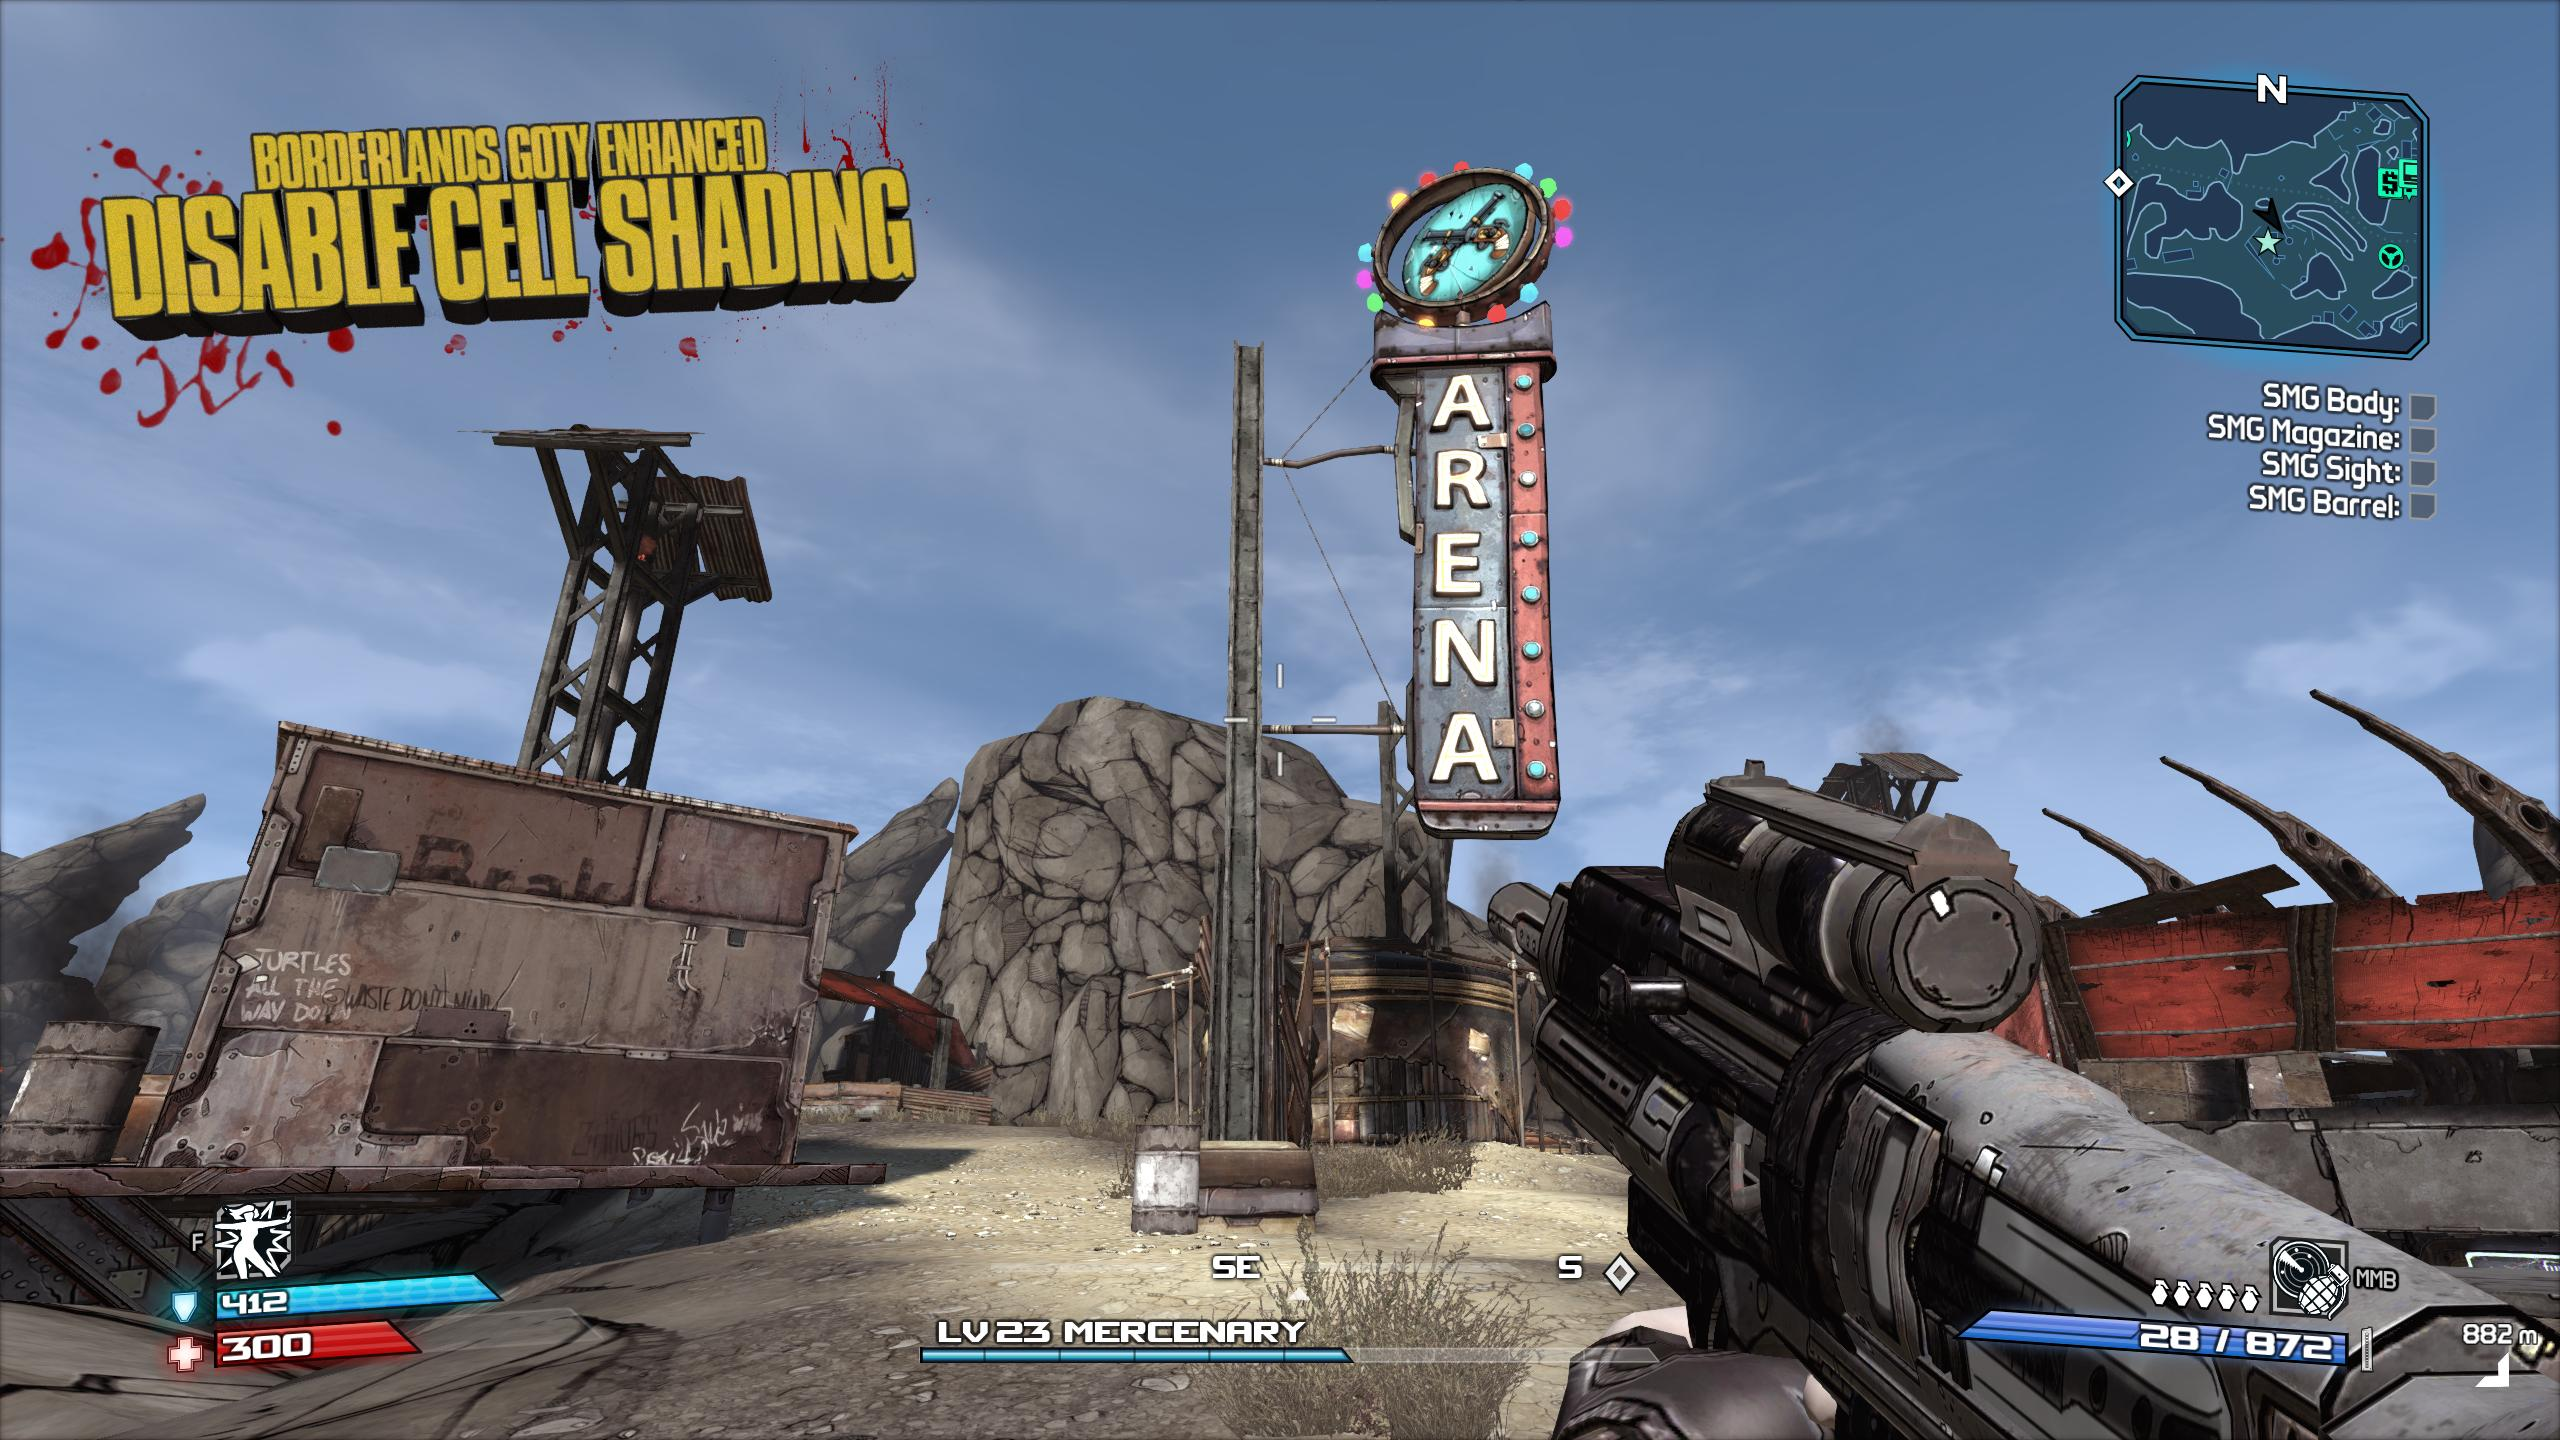
\includegraphics[width=0.4\linewidth]{image2.jpg} & Borderlands did it for fun \\
      \hline
      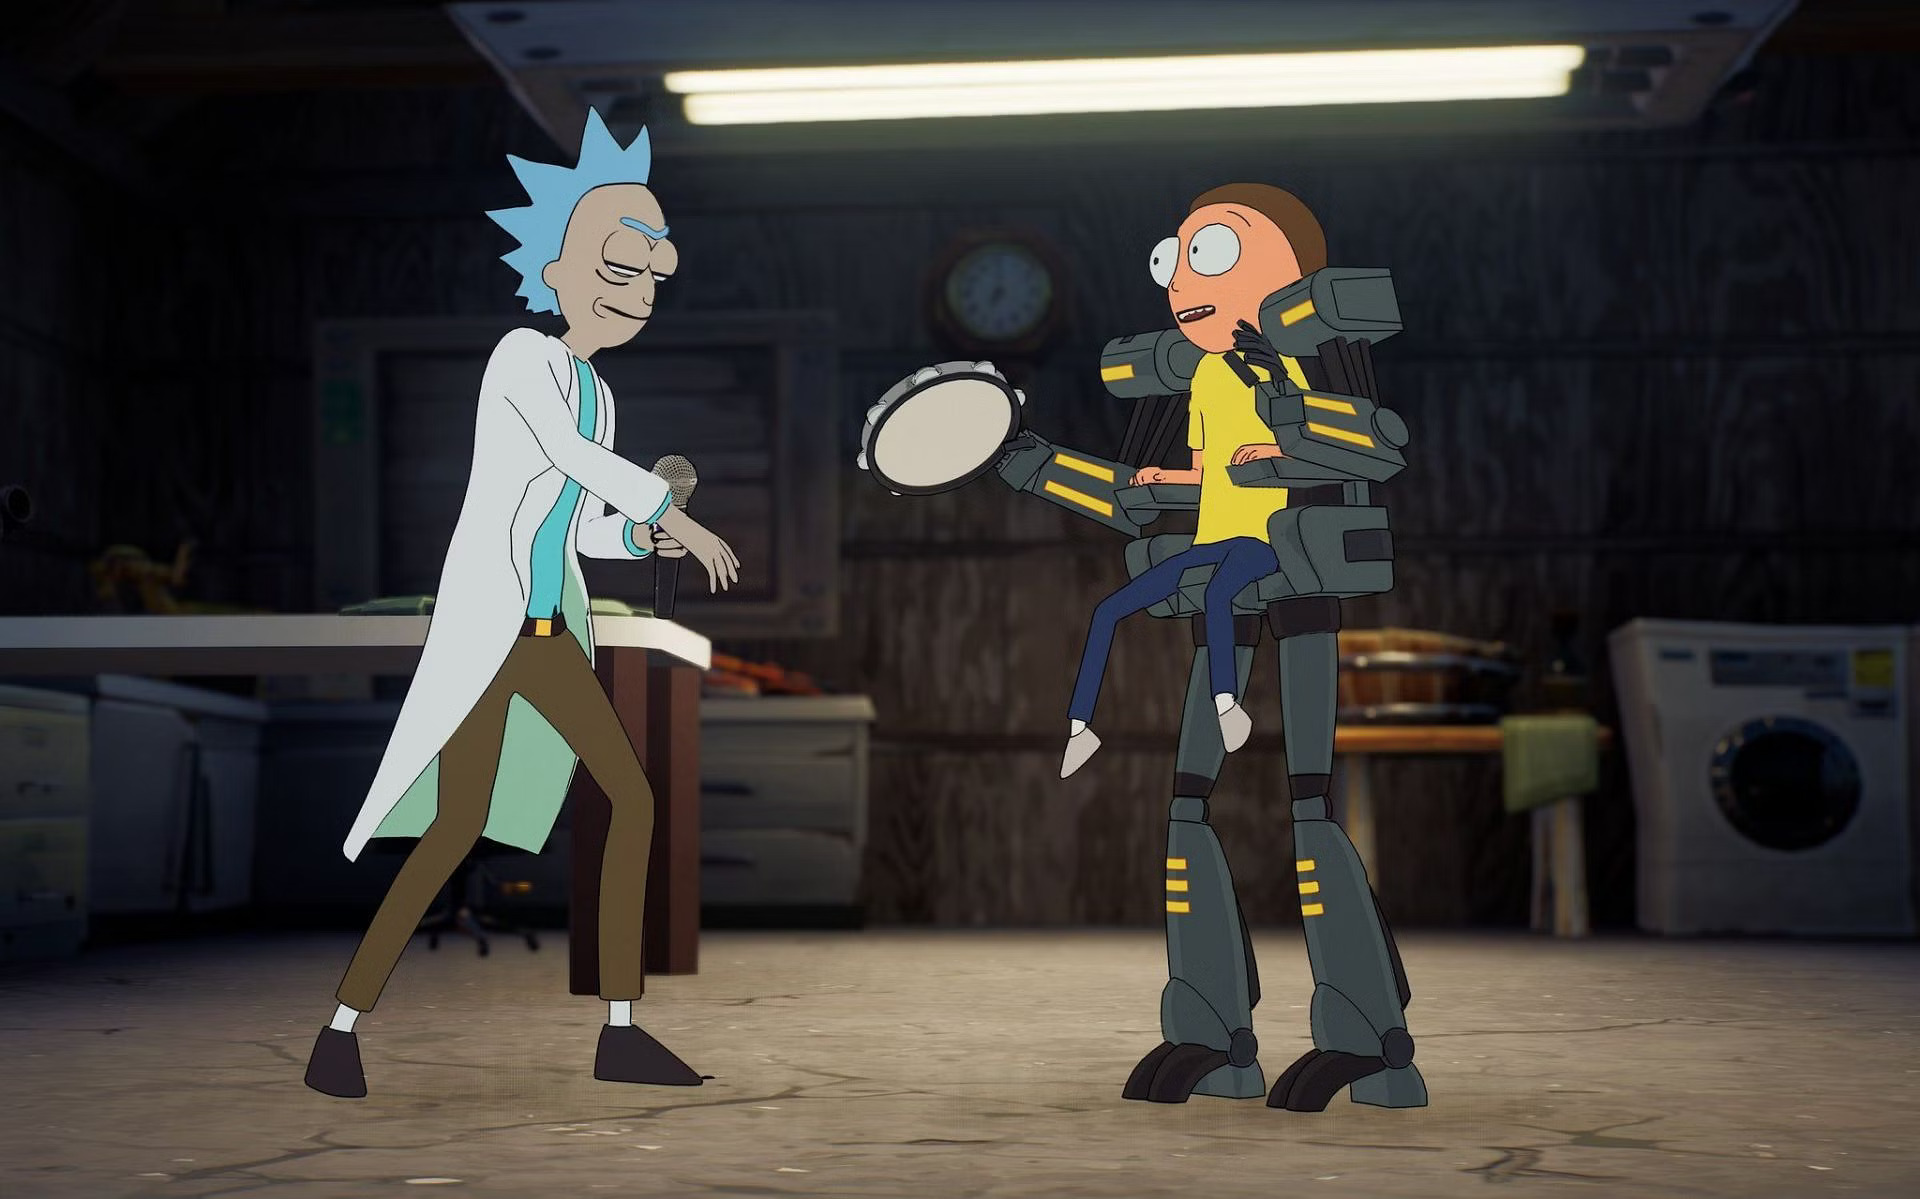
\includegraphics[width=0.4\linewidth]{image3.jpg} & Fortnite \\
      \hline
    \end{tabular}
    \caption{Pictures of inspiration}
    \label{tab:references}
  \end{table}

\end{document}

